\documentclass{report}

\input{~/latex/template/preamble.tex}
\input{~/latex/template/macros.tex}

\title{\Huge\textbf{Karaoke Management System Group Project}\\[1em] 
\Huge ER Diagram}

\author{
    \Large Matt Warner \and
    \Large Sang Pham \and
    \Large James Bolla \and
    \Large Emanuel Slaughter \and
    \Large Ty Danan
}

\date{\huge{}}
\pagestyle{fancy}
\fancyhf{}
\rhead{}
\lhead{\leftmark}
\cfoot{\thepage}
% \usepackage[default]{sourcecodepro} \usepackage[T1]{fontenc}

\pgfpagesdeclarelayout{boxed}
{
  \edef\pgfpageoptionborder{0pt}
  \pgfpagesphysicalpageoptions
  {%
    logical pages=1,%
  }
  \pgfpageslogicalpageoptions{1}
  {
    border code=\pgfsetlinewidth{1.5pt}\pgfstroke,%
    border shrink=\pgfpageoptionborder,%
    resized width=.95\pgfphysicalwidth,%
    resized height=.95\pgfphysicalheight,%
    center=\pgfpoint{.5\pgfphysicalwidth}{.5\pgfphysicalheight}%
  }%
}

\pgfpagesuselayout{boxed}

\begin{document}
    \maketitle
    \begin{center}
    \vspace*{\fill}
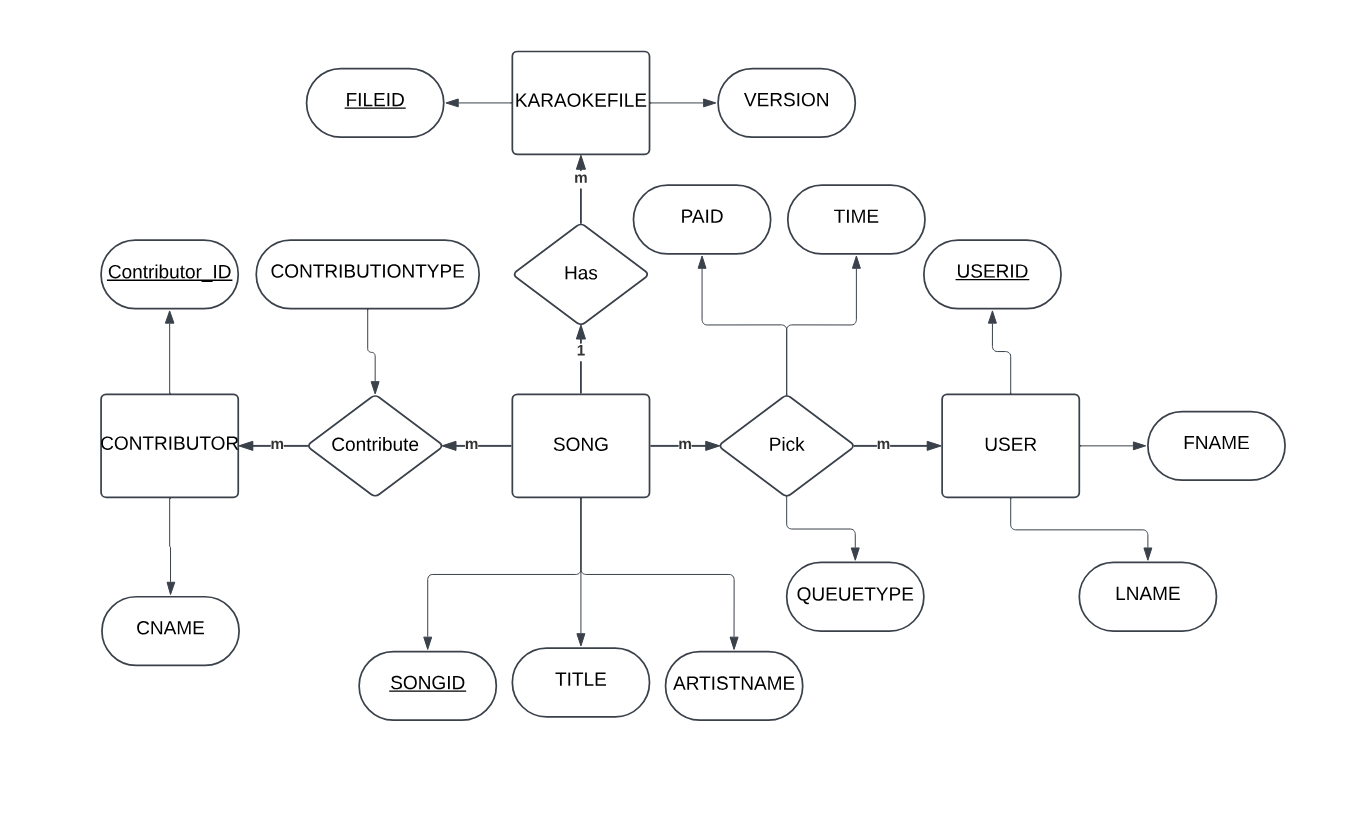
\includegraphics[width=1.1\textwidth]{ /home/matt/niu/fall24/cs466/proj/erd.png }
\vspace*{\fill}
    \end{center}
\newpage
\section{Entities \& Atributes}
\begin{itemize}
    \item \textbf{USER}
        \begin{itemize}[label=$\circ$]
            \item \texttt{\underline{USERID}} \ - \ A users unique identification number (primary key).
            \item \texttt{FNAME} \ - \ The users first name.
            \item \texttt{LNAME} \ - \ The users last name.
        \end{itemize}
    \item \texttt{SONG} 
        \begin{itemize}[label=$\circ$]
            \item \texttt{\underline{SONGID}} \ - \ A songs Unique identifer (primary key).
            \item \texttt{TITLE} \ - \ The name of the song.
            \item \texttt{ARTISTNAME} \ - \ The songs artist.
        \end{itemize}
    \item \texttt{CONTRIBUTOR}
        \begin{itemize}[label=$\circ$]
            \item \texttt{\underline{CONTRIBUTORID}} A contributors unique identifier.
            \item \texttt{\underline{CNAME}} \ - \ A contributors first and last name.
        \end{itemize}
        \item \texttt{KARAOKEFILE}
        \begin{itemize}[label=$\circ$]
            \item \texttt{\underline{FILEID}} \ - \  A files unique identification number (primary key).
            \item \texttt{VERSION} \ - \ The type of performance for the song in the file.
        \end{itemize}
\end{itemize}
\section{Relationships \& Cardinality}
\subsection{\textit{\textbf{Pick}}}
    This is a binary relationship between \texttt{USER} and \texttt{SONG}. \\
    \texttt{USER} \textit{picks} \texttt{SONG}.
    \bigbreak \noindent
    \underline{\textbf{Intersection data}}
    \begin{itemize}
        \item \texttt{TIME} \ - \ The time the user picks a song.
        \item \texttt{QUEUETYPE} \ - \ The type of queue (free or paid) that the user is placed in.
        \item \texttt{PAID}: The Amount paid by a user, which determines where they will end up in the queue.
    \end{itemize}
    \underline{\textbf{Cardinality}}
    \bigbreak \noindent
    Many-to-Many
    \begin{itemize}
        \item A single \texttt{USER} can pick multiple \texttt{SONG}'s.
        \item A single \texttt{SONG} can be picked by multiple \texttt{USER}'s.
    \end{itemize}
    \hline
    \subsection{Contribute}
    This is a binary relationship between \texttt{CONTRIBUTOR} and \texttt{SONG}.
    \bigbreak \noindent
    \underline{\textbf{Intersection data}}
    \begin{itemize}
        \item \texttt{CONTRIBUTIONTYPE} \ - \ This is the type of contribution that a contributor made to the song.
    \end{itemize}
    \underline{\textbf{Cardinality}}
    \begin{itemize}
        \item A single contributor can contribute to many songs.
        \item A single song can be contributed to by many contributors.
    \end{itemize}
    \subsection{ \textit{\textbf{Has}}} 
    This is a binary relationship between \texttt{KARAOKEFILE} and \texttt{SONG} \vspace{4mm} \\
    \texttt{SONG} \textit{has} \texttt{KARAOKEFILE}.
    \bigbreak \noindent
    \underline{\textbf{Intersection data}}
    \begin{itemize}
        \item None
    \end{itemize}
    \bigbreak \noindent
    \underline{\textbf{Cardinality}}
    \begin{itemize}
        \item A single song can have \textit{\textbf{many}} files.
        \item A single file can only have \textit{\textbf{one}} song.
    \end{itemize}
\end{document}

